\documentclass[tikz,border=4pt]{standalone}
\usepackage{libertine}
\usetikzlibrary{arrows.meta,calc,positioning,fit,backgrounds,shapes.geometric}
\definecolor{paperink}{HTML}{263441}
\definecolor{papermuted}{HTML}{647481}
\definecolor{paperline}{HTML}{CCD5DB}
\definecolor{paperblue}{HTML}{2D5F91}
\definecolor{paperbluefill}{HTML}{EFF5FA}
\definecolor{paperorange}{HTML}{B66731}
\definecolor{paperorangefill}{HTML}{FCF4EB}
\definecolor{papergreen}{HTML}{3F7558}
\definecolor{papergreenfill}{HTML}{EFF6F1}
\tikzset{
  papertext/.style={font=\footnotesize, text=paperink},
  papermini/.style={font=\scriptsize, text=papermuted},
  paneltitle/.style={font=\footnotesize\bfseries, text=paperink},
  bluebox/.style={draw=paperblue, fill=paperbluefill, rounded corners=1pt,
    line width=.6pt, font=\footnotesize, text=paperink, align=center,
    inner xsep=6pt, inner ysep=5pt},
  orangebox/.style={draw=paperorange, fill=paperorangefill, rounded corners=1pt,
    line width=.6pt, font=\footnotesize, text=paperink, align=center,
    inner xsep=6pt, inner ysep=5pt},
  greenbox/.style={draw=papergreen, fill=papergreenfill, rounded corners=1pt,
    line width=.6pt, font=\footnotesize, text=paperink, align=center,
    inner xsep=6pt, inner ysep=5pt},
  graybox/.style={draw=paperline, fill=white, rounded corners=1pt,
    line width=.6pt, font=\footnotesize, text=paperink, align=center,
    inner xsep=6pt, inner ysep=5pt},
  orangeflow/.style={-{Stealth[length=2mm]}, draw=paperorange, line width=1pt},
  blueflow/.style={-{Stealth[length=2mm]}, draw=paperblue, line width=1.15pt},
  greenflow/.style={-{Stealth[length=2mm]}, draw=papergreen, line width=1pt},
  grayflow/.style={-{Stealth[length=1.8mm]}, draw=papermuted, line width=.65pt}
}

\begin{document}
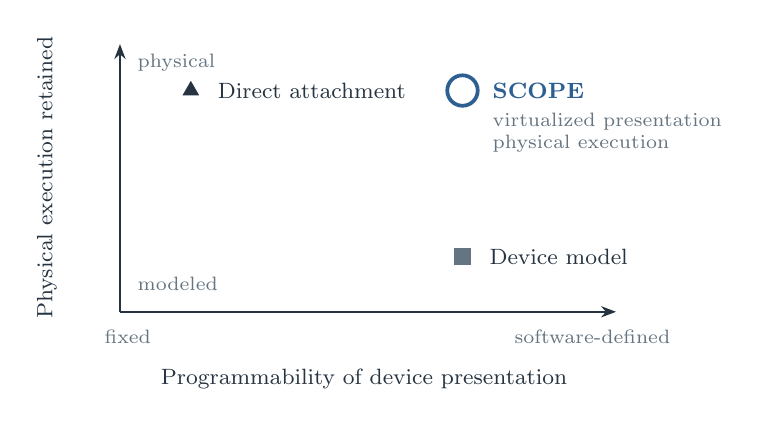
\begin{tikzpicture}[x=1cm,y=1cm]
  \draw[paperink, line width=.75pt, -{Stealth[length=1.9mm]}]
    (1.05,.75) -- (7.35,.75);
  \draw[paperink, line width=.75pt, -{Stealth[length=1.9mm]}]
    (1.05,.75) -- (1.05,4.15);
  \node[papermini, anchor=north] at (1.15,.64) {fixed};
  \node[papermini, anchor=north] at (7.05,.64) {software-defined};
  \node[papertext, anchor=north] at (4.15,.14)
    {Programmability of device presentation};
  \node[papermini, anchor=west] at (1.15,1.10) {modeled};
  \node[papermini, anchor=west] at (1.15,3.92) {physical};
  \node[papertext, rotate=90] at (.12,2.45)
    {Physical execution retained};

  \node[regular polygon, regular polygon sides=3, fill=paperink,
    minimum size=7pt, inner sep=0pt] at (1.95,3.56) {};
  \node[papertext, anchor=west] at (2.17,3.56) {Direct attachment};

  \node[rectangle, fill=papermuted, minimum width=6pt,
    minimum height=6pt, inner sep=0pt] at (5.4,1.45) {};
  \node[papertext, anchor=west] at (5.62,1.45) {Device model};

  \node[circle, draw=paperblue, fill=white, line width=1.35pt,
    minimum size=11pt, inner sep=0pt] at (5.4,3.56) {};
  \node[font=\footnotesize\bfseries, text=paperblue, anchor=west]
    at (5.66,3.56) {SCOPE};
  \node[papermini, anchor=west] at (5.66,3.17)
    {virtualized presentation};
  \node[papermini, anchor=west] at (5.66,2.88)
    {physical execution};
\end{tikzpicture}
\end{document}
